% Options for packages loaded elsewhere
\PassOptionsToPackage{unicode}{hyperref}
\PassOptionsToPackage{hyphens}{url}
\PassOptionsToPackage{dvipsnames,svgnames,x11names}{xcolor}
%
\documentclass[
  letterpaper,
  DIV=11,
  numbers=noendperiod]{scrartcl}

\usepackage{amsmath,amssymb}
\usepackage{iftex}
\ifPDFTeX
  \usepackage[T1]{fontenc}
  \usepackage[utf8]{inputenc}
  \usepackage{textcomp} % provide euro and other symbols
\else % if luatex or xetex
  \usepackage{unicode-math}
  \defaultfontfeatures{Scale=MatchLowercase}
  \defaultfontfeatures[\rmfamily]{Ligatures=TeX,Scale=1}
\fi
\usepackage{lmodern}
\ifPDFTeX\else  
    % xetex/luatex font selection
\fi
% Use upquote if available, for straight quotes in verbatim environments
\IfFileExists{upquote.sty}{\usepackage{upquote}}{}
\IfFileExists{microtype.sty}{% use microtype if available
  \usepackage[]{microtype}
  \UseMicrotypeSet[protrusion]{basicmath} % disable protrusion for tt fonts
}{}
\makeatletter
\@ifundefined{KOMAClassName}{% if non-KOMA class
  \IfFileExists{parskip.sty}{%
    \usepackage{parskip}
  }{% else
    \setlength{\parindent}{0pt}
    \setlength{\parskip}{6pt plus 2pt minus 1pt}}
}{% if KOMA class
  \KOMAoptions{parskip=half}}
\makeatother
\usepackage{xcolor}
\usepackage[right=1in,left=1in]{geometry}
\setlength{\emergencystretch}{3em} % prevent overfull lines
\setcounter{secnumdepth}{5}
% Make \paragraph and \subparagraph free-standing
\ifx\paragraph\undefined\else
  \let\oldparagraph\paragraph
  \renewcommand{\paragraph}[1]{\oldparagraph{#1}\mbox{}}
\fi
\ifx\subparagraph\undefined\else
  \let\oldsubparagraph\subparagraph
  \renewcommand{\subparagraph}[1]{\oldsubparagraph{#1}\mbox{}}
\fi


\providecommand{\tightlist}{%
  \setlength{\itemsep}{0pt}\setlength{\parskip}{0pt}}\usepackage{longtable,booktabs,array}
\usepackage{calc} % for calculating minipage widths
% Correct order of tables after \paragraph or \subparagraph
\usepackage{etoolbox}
\makeatletter
\patchcmd\longtable{\par}{\if@noskipsec\mbox{}\fi\par}{}{}
\makeatother
% Allow footnotes in longtable head/foot
\IfFileExists{footnotehyper.sty}{\usepackage{footnotehyper}}{\usepackage{footnote}}
\makesavenoteenv{longtable}
\usepackage{graphicx}
\makeatletter
\def\maxwidth{\ifdim\Gin@nat@width>\linewidth\linewidth\else\Gin@nat@width\fi}
\def\maxheight{\ifdim\Gin@nat@height>\textheight\textheight\else\Gin@nat@height\fi}
\makeatother
% Scale images if necessary, so that they will not overflow the page
% margins by default, and it is still possible to overwrite the defaults
% using explicit options in \includegraphics[width, height, ...]{}
\setkeys{Gin}{width=\maxwidth,height=\maxheight,keepaspectratio}
% Set default figure placement to htbp
\makeatletter
\def\fps@figure{htbp}
\makeatother
\newlength{\cslhangindent}
\setlength{\cslhangindent}{1.5em}
\newlength{\csllabelwidth}
\setlength{\csllabelwidth}{3em}
\newlength{\cslentryspacingunit} % times entry-spacing
\setlength{\cslentryspacingunit}{\parskip}
\newenvironment{CSLReferences}[2] % #1 hanging-ident, #2 entry spacing
 {% don't indent paragraphs
  \setlength{\parindent}{0pt}
  % turn on hanging indent if param 1 is 1
  \ifodd #1
  \let\oldpar\par
  \def\par{\hangindent=\cslhangindent\oldpar}
  \fi
  % set entry spacing
  \setlength{\parskip}{#2\cslentryspacingunit}
 }%
 {}
\usepackage{calc}
\newcommand{\CSLBlock}[1]{#1\hfill\break}
\newcommand{\CSLLeftMargin}[1]{\parbox[t]{\csllabelwidth}{#1}}
\newcommand{\CSLRightInline}[1]{\parbox[t]{\linewidth - \csllabelwidth}{#1}\break}
\newcommand{\CSLIndent}[1]{\hspace{\cslhangindent}#1}

\usepackage{booktabs}
\usepackage{longtable}
\usepackage{array}
\usepackage{multirow}
\usepackage{wrapfig}
\usepackage{float}
\usepackage{colortbl}
\usepackage{pdflscape}
\usepackage{tabu}
\usepackage{threeparttable}
\usepackage{threeparttablex}
\usepackage[normalem]{ulem}
\usepackage{makecell}
\usepackage{xcolor}
\usepackage{colortbl}
\KOMAoption{captions}{tableheading}
\makeatletter
\makeatother
\makeatletter
\makeatother
\makeatletter
\@ifpackageloaded{caption}{}{\usepackage{caption}}
\AtBeginDocument{%
\ifdefined\contentsname
  \renewcommand*\contentsname{Table of contents}
\else
  \newcommand\contentsname{Table of contents}
\fi
\ifdefined\listfigurename
  \renewcommand*\listfigurename{List of Figures}
\else
  \newcommand\listfigurename{List of Figures}
\fi
\ifdefined\listtablename
  \renewcommand*\listtablename{List of Tables}
\else
  \newcommand\listtablename{List of Tables}
\fi
\ifdefined\figurename
  \renewcommand*\figurename{Figure}
\else
  \newcommand\figurename{Figure}
\fi
\ifdefined\tablename
  \renewcommand*\tablename{Table}
\else
  \newcommand\tablename{Table}
\fi
}
\@ifpackageloaded{float}{}{\usepackage{float}}
\floatstyle{ruled}
\@ifundefined{c@chapter}{\newfloat{codelisting}{h}{lop}}{\newfloat{codelisting}{h}{lop}[chapter]}
\floatname{codelisting}{Listing}
\newcommand*\listoflistings{\listof{codelisting}{List of Listings}}
\makeatother
\makeatletter
\@ifpackageloaded{caption}{}{\usepackage{caption}}
\@ifpackageloaded{subcaption}{}{\usepackage{subcaption}}
\makeatother
\makeatletter
\@ifpackageloaded{tcolorbox}{}{\usepackage[skins,breakable]{tcolorbox}}
\makeatother
\makeatletter
\@ifundefined{shadecolor}{\definecolor{shadecolor}{rgb}{.97, .97, .97}}
\makeatother
\makeatletter
\makeatother
\makeatletter
\makeatother
\ifLuaTeX
  \usepackage{selnolig}  % disable illegal ligatures
\fi
\IfFileExists{bookmark.sty}{\usepackage{bookmark}}{\usepackage{hyperref}}
\IfFileExists{xurl.sty}{\usepackage{xurl}}{} % add URL line breaks if available
\urlstyle{same} % disable monospaced font for URLs
\hypersetup{
  pdftitle={How Do Household Energy Transitions Work?},
  pdfauthor={Jill Baumgartner (Co-PI); Sam Harper (Co-PI)},
  colorlinks=true,
  linkcolor={blue},
  filecolor={Maroon},
  citecolor={Blue},
  urlcolor={Blue},
  pdfcreator={LaTeX via pandoc}}

\title{How Do Household Energy Transitions Work?}
\author{Jill Baumgartner (Co-PI) \and Sam Harper (Co-PI)}
\date{2024-04-01}

\begin{document}
\maketitle
\ifdefined\Shaded\renewenvironment{Shaded}{\begin{tcolorbox}[enhanced, breakable, borderline west={3pt}{0pt}{shadecolor}, sharp corners, boxrule=0pt, frame hidden, interior hidden]}{\end{tcolorbox}}\fi

\renewcommand*\contentsname{Table of contents}
{
\hypersetup{linkcolor=}
\setcounter{tocdepth}{3}
\tableofcontents
}
\begin{verbatim}
here() starts at /Users/samharper/git/bhet-report
\end{verbatim}

\begin{verbatim}
Automatically registered OSF personal access token
\end{verbatim}

\begin{verbatim}
-- Attaching core tidyverse packages ------------------------ tidyverse 2.0.0 --
v dplyr     1.1.4     v readr     2.1.5
v forcats   1.0.0     v stringr   1.5.1
v ggplot2   3.5.0     v tibble    3.2.1
v lubridate 1.9.3     v tidyr     1.3.1
v purrr     1.0.2     
-- Conflicts ------------------------------------------ tidyverse_conflicts() --
x dplyr::filter() masks stats::filter()
x dplyr::lag()    masks stats::lag()
i Use the conflicted package (<http://conflicted.r-lib.org/>) to force all conflicts to become errors

Attaching package: 'kableExtra'


The following object is masked from 'package:dplyr':

    group_rows


Version 2.0.0 of `modelsummary`, to be released soon, will introduce a
  breaking change: The default table-drawing package will be `tinytable`
  instead of `kableExtra`. All currently supported table-drawing packages
  will continue to be supported for the foreseeable future, including
  `kableExtra`, `gt`, `huxtable`, `flextable, and `DT`.
  
  You can always call the `config_modelsummary()` function to change the
  default table-drawing package in persistent fashion. To try `tinytable`
  now:
  
  config_modelsummary(factory_default = 'tinytable')
  
  To set the default back to `kableExtra`:
  
  config_modelsummary(factory_default = 'kableExtra')
\end{verbatim}

\hypertarget{abstract}{%
\subsection*{Abstract}\label{abstract}}

\hypertarget{introduction}{%
\subsubsection*{Introduction}\label{introduction}}

\hypertarget{methods}{%
\subsubsection*{Methods}\label{methods}}

\hypertarget{results}{%
\subsubsection*{Results}\label{results}}

\hypertarget{conclusions}{%
\subsubsection*{Conclusions}\label{conclusions}}

\hypertarget{introduction-1}{%
\section{Introduction}\label{introduction-1}}

China is deploying an ambitious policy to transition up to 70\% of
households in northern China to clean space heating, including Beijing.
To meet this target the Beijing municipal government announced a
two-pronged program that designates coal-restricted areas and
simultaneously offers subsidies to night-time electricity rates and for
the purchase and installation of electric-powered, air-source heat pumps
to replace traditional coal-heating stoves. The program is being rolled
out on a village-by-village basis; however there is uncertainty as to
when villages will receive the program. The variability in when the
policy is applied to each village allows us to treat the roll-out of the
program as a quasi-randomized intervention. Households may also be
differentially affected by this program due to factors such as financial
constraints, preferences and social capital, and there is uncertainty
about whether and how this intervention may affect indoor and outdoor
air pollution, as well as health behaviors and health outcomes.

\hypertarget{background}{%
\section{Background}\label{background}}

\hypertarget{context-for-the-policy}{%
\subsection{Context for the policy}\label{context-for-the-policy}}

Household coal burning has been a major contributor to indoor and
outdoor air pollution in northern China, especially in winter. Prior to
2016, coal fuel was used to meet over 80\% of northern China's space
heating demand (ref NRDC doc). Household coal-fuelled heaters, common in
peri-urban and rural areas without access to centralized heating, burned
approximately half of the over 400 million tons of coal used for space
heating (ref NRDC doc) and contributed to \textasciitilde30\% of
northern China's wintertime air pollution. {[}{[}{[}something on health
impacts{]}{]}{]}

Replacing household coal stoves with clean heating alternatives was
considered a potentially impactful intervention to reduce outdoor PM2.5
and its health impacts.

A number of clean heating options including electric heat pumps, gas
heaters, and electric resistance heaters with thermal storage were
widely promoted by the Chinese government (ref NRDC doc).

By 2021, over 36 million households in northern China were treated by
the policy and an estimated 21 million more households were expected to
be treated by 2025. Whether this large-scale energy policy yielded
health benefits remains a critical and unresolved question.

\hypertarget{prior-evidence-of-household-energy-interventions-and-air-pollution}{%
\subsection{Prior evidence of household energy interventions and air
pollution}\label{prior-evidence-of-household-energy-interventions-and-air-pollution}}

See
\href{https://onlinelibrary.wiley.com/doi/epdf/10.1111/ina.12958}{report}
from Woolley et al (Woolley et al. 2022)

\hypertarget{prior-evidence-on-clean-energy-interventions}{%
\subsection{Prior evidence on clean energy
interventions}\label{prior-evidence-on-clean-energy-interventions}}

Most previous health assessments of household energy technologies have
focused on cookstoves and not heating stoves. Randomized trials of less
polluting cookstoves indicate a cardiovascular benefit of clean heating
energy transition. In Guatemala, a chimney stove intervention lowered
exposure to air pollution and reduced the occurrence of nonspecific
ST-segment depression, an indicator of health conditions including
myocardial ischemia, in older women. That same study and other trials in
Nigeria and Ghana observed reductions in blood pressure (range: −3.7 to
−1.3mmHg) in women assigned gas, ethanol, or improved combustion biomass
stoves, and are supported by non-randomized, controlled intervention
studies in Nicaragua and Bolivia (blood pressure reductions ranging −5.9
to −5.5mmHg). In contrast, a recent multi-country randomized trial did
not observe a protective effect of gas stoves on gestational blood
pressure despite large reductions in indoor and personal exposures to
PM2.5, though the participants were younger (mean age: 25y) than in
studies showing a blood pressure benefit of intervention (mean ages: 28
to 53y).

The few previous evaluations of household energy policies, mostly in
high-income countries, have also indicated some health benefit, though
many did not control for secular changes in health over time.
Residential wood-burning bans were associated with reductions in
cardiovascular hospitalizations (-7\%) in California's San Joaquin
Valley, and with reduced cardiovascular (17.9\%) and respiratory
(−22.8\%) mortality in Launceston, Tasmania (Australia), though neither
study fully controlled for secular improvements in health. Most relevant
to our study are two quasi-experimental assessments of coal replacement
policies. Small decreases in chronic lung diseases (-3.0 to -1.1\%) were
observed in a multi-city cohort of 8524 Chinese adults in cities where
the coal-to-clean energy policy was piloted compared with adults in
cities not included in the pilot. The study observed no change in
physician-diagnosed cardiovascular diseases, potentially due to the only
one-year post-policy period or confounding by other city-wide air
quality and health-related policies. In a population-based study in
Ireland, reductions in respiratory mortality were observed, but no
effect was found for cardiovascular mortality after accounting for
secular changes in health.

\hypertarget{importance-of-understanding-mechanisms-through-which-policies-may-affect-outcomes.}{%
\subsection{Importance of understanding mechanisms through which
policies may affect
outcomes.}\label{importance-of-understanding-mechanisms-through-which-policies-may-affect-outcomes.}}

\hypertarget{specific-aims-and-overarching-approach}{%
\section{Specific Aims and Overarching
Approach}\label{specific-aims-and-overarching-approach}}

This study used three data collection campaigns in winter 2018/19,
winter 2019/20, and winter 2021/22, as well as a partial campaign in
winter 2020/21 to advance the following aims:

\begin{enumerate}
\def\labelenumi{\arabic{enumi}.}
\item
  Estimate how much of the policy's overall effect on health, including
  respiratory symptoms and cardiovascular outcomes (blood pressure,
  central hemodynamics, blood inflammatory and oxidative stress
  markers), can be attributed to its impact on changes in PM2.5;
\item
  Quantify the impact of the policy on outdoor air quality and personal
  air pollution exposures, and specifically the source contribution from
  household coal burning (Previously Aim 3);
\item
  Quantify the contribution of changes in the chemical composition of
  PM2.5 from different sources to the overall effect on health outcomes
  (Previously Aim 2).
\end{enumerate}

\hypertarget{study-design-and-methods}{%
\section{Study Design and Methods}\label{study-design-and-methods}}

\hypertarget{location-context-and-recruitment}{%
\subsection{Location, context, and
recruitment}\label{location-context-and-recruitment}}

In December 2018 we recruited 50 villages across 4 administrative
divisions of peri-urban Beijing to participate in our study. Villages
were selected on the basis of their residents primarily using household
coal and/or biomass stoves, and because roughly half of the villages
were expected to enter into the CBHP policy over the course of our
study. We used local guides in each village to help determine a roster
of households that were not vacant during the winter months, from which
we selected households to recruit for participation.

We recruited approximately 20 households in each village and randomly
selected one eligible person from each household to participate.
Participants were eligible to participate if they were over 40 years
old, lived in the study villages, were not planning to move out of the
village in the next year, and were not on current immunotherapy or
treatment with corticosteroids. Research staff introduced the study and
its measurements to an eligible person in each household and answered
any questions related to the study. All participants provided written
informed consent prior to joining the study. The study protocols were
approved by research ethics boards at Peking University
(IRB00001052-18090) and McGill University (A08-E53-18B).

\hypertarget{measures}{%
\subsection{Measures}\label{measures}}

\hypertarget{village-level}{%
\subsubsection{Village level:}\label{village-level}}

\begin{itemize}
\tightlist
\item
  Outdoor air pollution
\item
  Qualitative and quantitative information on current policies/programs
  with government funding from local leaders
\end{itemize}

\hypertarget{household-level}{%
\subsubsection{Household level:}\label{household-level}}

\begin{itemize}
\tightlist
\item
  Questionnaire to assess energy use and related expenditures
\item
  Indoor air temperature (\textasciitilde75\% of homes for 2+ winter
  months)
\item
  Indoor PM2.5 in \textasciitilde50\% of study homes
\item
  Electricity use based on meters
\end{itemize}

\hypertarget{individual-level}{%
\subsubsection{Individual level:}\label{individual-level}}

\textbf{Questionnaires on health status, behaviors, and medication}

Field staff administered questionnaires to assess household demographic
information, household assets, house structure, stove and fuel use
patterns (including a complete roster of heating methods and their
contributions in each room), and smoking. We used Surveybe
computer-assisted personal interview (CAPI) software to collect survey
data via handheld electronic tablets. Questions were read to
participants in Mandarin-Chinese, and their responses were recorded into
tablets.

The questionnaire and other study measurements were tested prior to the
start of data collection for this study in 12 households located in
Beijing village that was eligible for our study but was instead selected
for testing prior to the study start. We used the test village to assess
whether the questions were understandable and interpreted as intended
and to identify any problems with the study measurements or their
implementation. Study protocols were subsequently adapted prior to the
start of data collection.

\textbf{Personal exposures to PM2.5 and black carbon (50\% of
participants)}\footnote{SH: Taken from Appendix from (Li et al. 2022),
  needs to be re-written}

To measure personal exposure we used two types of samplers: Personal
Exposure Monitors (PEMs, Apex Pro; Casella, UK) and Ultrasonic Personal
Aerosol Samplers (UPAS, Access Sensor Technologies, Fort Collins, CO,
USA). PEMs actively sampled at a flow rate of 1.8 L/min, and UPAS was at
1.0 L/min (Volckens et al. 2017). Both samplers housed 37 mm PTFE
filters (VWR, 2.0-μm pore size) and were equipped with a cyclone inlet
with a 2.5 μm cutpoint. Sampler flow rates were calibrated the night
before deployment and also measured after the sampling period. Few
post-sampling measurements (16 out of 494, 3\%) deviated from the target
flow rate by \textgreater10\%. Participants were instructed to wear a
small waistpack (for the PEM and sampling pump) or an arm bag (for the
UPAS) for 24 hours, which they could place within 2 meters while
sleeping, sitting, or bathing. Field blanks were collected at a rate of
\textasciitilde10\% in each village. All filters were placed in
individually labeled Petri dishes, sealed in plastic bags, and then
transported to a field laboratory and immediately stored in a -20°C
freezer. Following completion of the field sampling campaign, the
samples and blanks were transported to Colorado State University, where
they were stored in a -20°C freezer prior to PM\textsubscript{2.5} mass
measurement and BC analysis.

All filters were placed in an environmentally-controlled equilibration
chamber (21-22 °C, 30-34\% relative humidity) for at least 24 hours
before tare and gross weighing. Before each weight was taken, filters
were discharged on a polonium-210 strip for at least 15 seconds. Filters
were weighed on a microbalance (Mettler Toledo Inc., XS3DU, USA) with
1-μg resolution in triplicate or more, until the differences among three
weights were less than 3 μg. The average of three readings was used to
determine filter mass, which was then blank-corrected using the median
value of blank filters {[}3 μg for UPAS-collected filters (53\% of
samples); 33 μg for PEM-collected filters (47\% of filter samples){]},
and PM2.5 concentrations were calculated by dividing the mass by the
sampled air volume.

Filters were analyzed for black carbon (BC) using an optical
transmissometer data acquisition system (SootScan\^{}TM OT21 Optical
Transmissometer; Magee Scientific, Berkeley, CA, USA). Light attenuation
through each filter was measured before and after sampling in the field.
To calculate BC mass, the difference between the pre- and post- light
attenuation was converted to a mass surface loading using the classical
Magee mass absorption cross-sections of 16.6 m2/g for the 880 nm channel
optical BC (Ahmed et al. 2009). BC concentrations were calculated by
multiplying surface loadings by the sampled surface area of the filters
(8.6 cm2 for UPAS-collected filters; 7.1 cm2 for PEM-collected filters),
correcting for the field blank mass using the median value of blanks
(0.31 μg for UPAS-collected filters; 0.01 μg for PEM-collected filters),
and finally dividing by the sampled air volume.

\begin{itemize}
\item
  Health measurements including blood pressure (all), self-reported
  respiratory symptoms (all), blood inflammatory and oxidative stress
  markers (\textasciitilde70\% in first two campaigns only), grip
  strength (\textasciitilde75\%), and airway inflammation
  (\textasciitilde20\%).
\item
  Field equipment (Figure)
\end{itemize}

\hypertarget{measuring-policy-impacts}{%
\subsection{Measuring policy impacts}\label{measuring-policy-impacts}}

To understand how Beijing's policy works we used a
difference-in-differences (DiD) design (Callaway 2020), leveraging the
staggered rollout of the policy across multiple villages to estimate its
impact on health outcomes and understand the mechanisms through which it
works. Simple comparisons of treated and untreated (i.e., control)
villages after the CBHP policy has been implemented are likely to be
biased by unmeasured village-level characteristics (e.g., migration,
average winter temperature) that are associated with health outcomes.
Similarly, comparisons of only treated villages before and after
exposure to the program are susceptible to bias by other factors
associated with changes in outcomes over time (i.e., secular trends,
impacts of the COVID-19 pandemic). By comparing \emph{changes} in
outcomes among treated villages to \emph{changes} in outcomes among
untreated villages, we can control for any unmeasured time-invariant
characteristics of villages as well as any general secular trends
affecting all villages that are unrelated to the policy

\begin{itemize}
\tightlist
\item
  DiD schematic (Figure)
\end{itemize}

\begin{figure}

{\centering 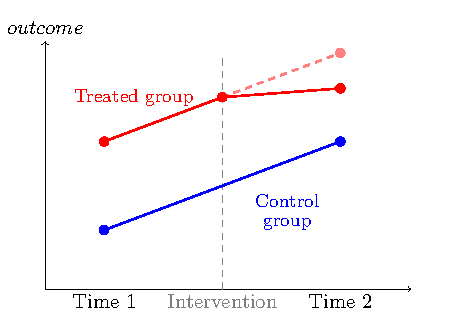
\includegraphics[width=0.7\textwidth,height=\textheight]{hei-report_files/figure-pdf/didfig-1.pdf}

}

\caption{Stylized example of difference-in-differences}

\end{figure}

The DiD design compares outcomes before and after an intervention in a
treated group relative to the same outcomes measured in a control group.
The control group trend provides the crucial ``counterfactual'' estimate
of what would have happened in the treated group had it not been
treated. By comparing each group to itself, this approach helps to
control for both measured and unmeasured fixed differences between the
treated and control groups. By measuring changes over time in outcomes
in the control group unaffected by the treatment, this approach also
controls for any unmeasured factors affecting outcome trends in both
treated and control groups. This is important since there are often many
potential factors affecting outcome trends that cannot be disentangled
from the policy if one only studies the treated group (as in a
traditional pre-post design).

The canonical DiD design (Card and Krueger 1994) compares two groups
(treated and control) at two different time periods (pre- and
post-intervention, Figure X). In the first time period both groups are
untreated, and in the second time period one group is exposed to the
intervention. If we assume that the differences between the groups would
have remained constant in the absence of the intervention (parallel
trends assumption), then an unbiased estimate of the impact of the
intervention in the post period can be calculated by subtracting the
pre-post difference in the untreated group from the pre-post difference
in the treated group.

However, when multiple groups are treated at different time periods, the
most common approach has been to use a two-way fixed effects model to
estimate the impact of the intervention which controls for secular
trends and differences between districts. However, recent evidence
suggests that the traditional two-way fixed effects estimation of the
treatment effect may be biased in the context of heterogeneous treatment
effects (Callaway and Sant'Anna 2021; Goodman-Bacon 2021)

\hypertarget{measuring-pathways-and-mechanisms}{%
\subsection{Measuring pathways and
mechanisms}\label{measuring-pathways-and-mechanisms}}

To estimate how much of the CBHP intervention may work through different
mechanisms, we used causal mediation analysis. Causal approaches to
mediation attempt to discern between, and clarify the necessary
assumptions for identifying, different kinds of mediated effects. Taking
as an example the DAG in \textbf{Figure X}, with \(T\) as the policy,
\(M\) as PM\textsubscript{2.5}, and \(Y\) as systolic blood pressure, we
can define the controlled direct effect (\(CDE\)) as the effect of the
CBHP policy on systolic blood pressure if we fix the value of
PM\textsubscript{2.5} to a certain reference level for the entire
population. For example, we can estimate the impact of the policy on
health outcomes while holding PM\textsubscript{2.5} at a uniform level
of average background exposure, or some other hypothetical level.

\begin{itemize}
\tightlist
\item
  Mediation DAG (Figure)
\end{itemize}

\begin{figure}

{\centering 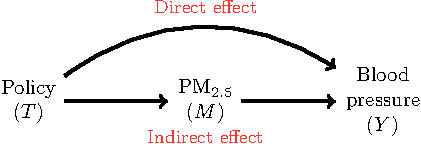
\includegraphics[width=0.7\textwidth,height=\textheight]{hei-report_files/figure-pdf/dag1-1.pdf}

}

\caption{Example of direct and indirect effects with outcome (\(Y\)),
treatment (\(T\)), and mediator (\(M\))}

\end{figure}

Although other mediated effects such as ``natural'' direct and indirect
effects are theoretically estimable (VanderWeele 2015), they involve
challenging ``cross-world'' assumptions that are difficult to anchor in
policy (Naimi et al. 2014). Other approaches to mechanisms have focused
on principal stratification (e.g., Zigler et al. 2016), although
conceptual difficulties with identifying the (unverifiable) principal
strata make it challenging for questions of mediation. Because
controlled direct effects are considered more directly policy relevant
for public health, we focus on estimating these mediated quantities.

\hypertarget{data-analysis}{%
\section{Data Analysis}\label{data-analysis}}

\hypertarget{total-effect}{%
\subsection{Total Effect}\label{total-effect}}

To estimate the total effect of the policy we used a DiD analysis that
accommodates staggered treatment rollout. To allow for heterogeneity in
the context of staggered rollout we used `extended' two-way fixed
effects (ETWFE) models (Wooldridge 2021) to estimate the total effect of
the CBHP policy. The mean outcome (replaced by a suitable link function
\(g(\cdot)\) for binary or count outcomes) was defined using a set of
linear predictors:

\begin{equation}\protect\hypertarget{eq-etwfe}{}{Y_{ijt}=g(\mu_{ijt}) = \alpha + \sum_{r=q}^{T} \beta_{r} d_{r} + \sum_{s=r}^{T} \gamma_{s} fs_{t}+ \sum_{r=q}^{T} \sum_{s=r}^{T} \tau_{rt} (d_{r} \times fs_{t}) + \varepsilon_{ijt}}\label{eq-etwfe}\end{equation}

where \(Y_{ijt}\) is the outcome for individual \(i\) in village \(j\)
at time \(t\), \(d_{r}\) represent treatment cohort dummies, i.e., fixed
effects for cohorts of villages that were first exposed to the policy at
the same time \(q\) (e.g., in 2019, 2020, or 2021), \(fs_{t}\) are time
fixed effects corresponding to different winter data collection
campaigns (2018-19, 2019-20, or 2021-22), and \(\tau_{rt}\) are the
cohort-time \emph{ATTs}. The ETWFE and other approaches that allow for
several (potentially heterogenous) treatment effects may also be
averaged to provide a weighted \(ATT\). Several potential possibilities
are feasible, including weighting by treatment cohorts or time since
policy adoption (Goin and Riddell 2023)

\hypertarget{mediation-analysis}{%
\subsection{Mediation Analysis}\label{mediation-analysis}}

As noted above, with respect to the mediation analysis we are chiefly
interested in the \(CDE\), which can be derived by adding relevant
mediators \(M\) to this model. If we also allow for exposure-mediator
interaction and potentially allow for adjustment for confounders \(W\)
of the mediator-outcome effect, we can extend equation
Equation~\ref{eq-etwfe} as follows:

\begin{equation}\protect\hypertarget{eq-etwfem}{}{
\begin{aligned}
Y_{ijt}=g(\mu_{ijt}) = \alpha + \sum_{r=q}^{T} \beta_{r} d_{r} + \sum_{s=r}^{T} \gamma_{s} fs_{t}+ \sum_{r=q}^{T} \sum_{s=r}^{T} \tau_{rt} (d_{r} \times fs_{t}) \\ + \delta M_{it} + \sum_{r=q}^{T} \sum_{s=r}^{T} \eta_{rt} (d_{r} \times fs_{t} \times M_{it}) + \zeta \mathbf{W} + \varepsilon_{ijt}
\end{aligned}
}\label{eq-etwfem}\end{equation}

where now \(\delta\) is the conditional effect of the mediator \(M\) at
the reference level of the treatment (again, represented via the series
of group-time interaction terms), and the collection of \(\eta\) terms
are coefficients for the product terms allowing for mediator-treatment
interaction. Finally, \(\zeta\) is a vector of coefficients for the set
of confounders contained within \(\mathbf{W}\).

As noted above, in the staggered DiD framework that allows for
heterogeneity we do not have a single treatment effect but a collection
of group-time treatment effects that may be averaged in different ways.
This extends to the estimation of the \(CDE\), in which case we will
also have several \(CDE\)s that can be averaged to make inferences about
the extent to which the policy's impact is mediated by
\emph{PM\textsubscript{2.5}}. Based on the setup in
Equation~\ref{eq-etwfem} the \(CDE\) is estimated as:
\(\delta + \eta_{rt}MT\). In the absence of interaction between the
exposure and the mediator (i.e., \(\eta_{rt}=0\)) the \(CDE\) will
simply be the estimated treatment effects
\(\sum_{r=q}^{T} \sum_{s=r}^{T} \tau_{rt}\), i.e., the effect of the
policy holding \(M\) constant. For a valid estimate of the \(CDE\) we
must account for confounding of the mediator-outcome effect, represented
by \(W\) in the equation above. Baseline measures of both the outcome
and the proposed mediators inherent in our DiD strategy will help to
reduce the potential for unmeasured confounding of the mediator-outcome
effect (Keele et al. 2015).

\hypertarget{results-1}{%
\section{Results}\label{results-1}}

Study flowchart

\begin{figure}

{\centering 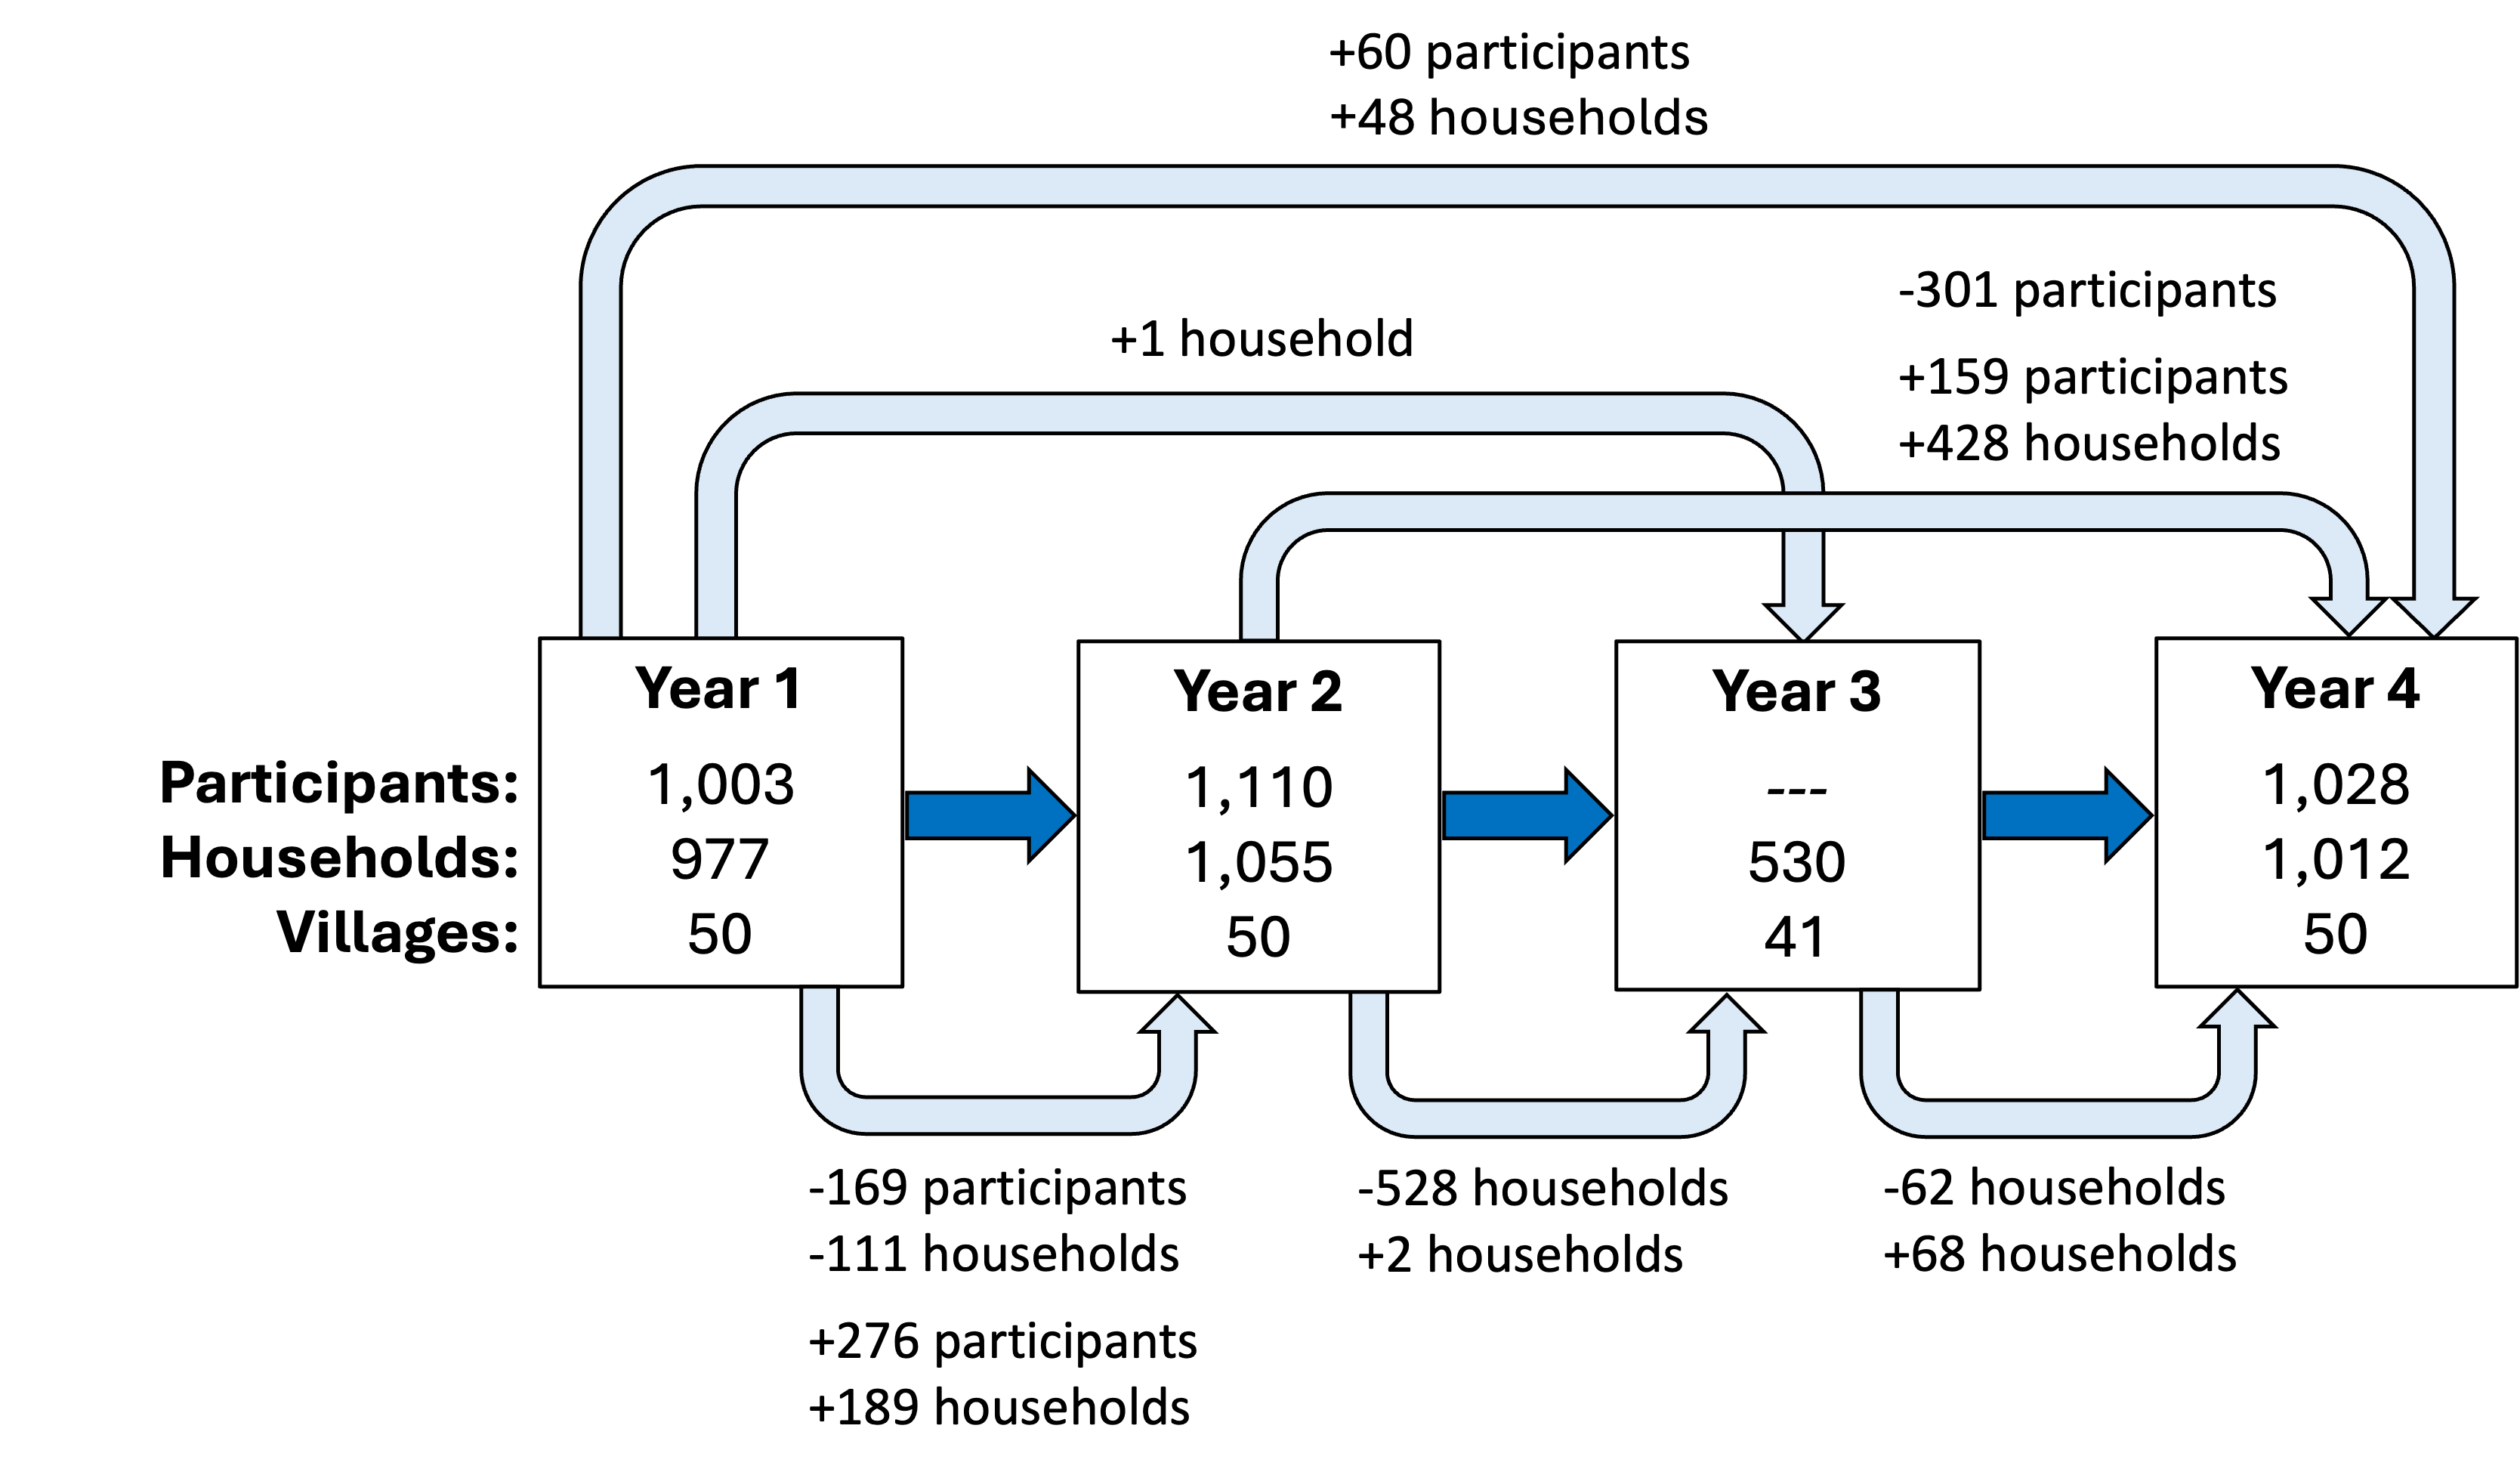
\includegraphics[width=1\textwidth,height=\textheight]{images/participation-flow-chart-Mar18.png}

}

\caption{\label{fig-flowchart}Flow chart of BHET study participation at
the participant, household, and village levels across study years.
Participation (number of units) in each study year is shown in the white
boxes. Additions (+) and losses (-) to the study sample between years
are indicated by the light blue arrows. Data collection was limited to
household- and village-level environmental measurements due to the
COVID-19 pandemic in year 3. We visited 530 households in 41 villages
before travel restrictions limited further data collection. This affects
the additions and losses to the study sample reported from years 2 to 3
and years 3 to 4.}

\end{figure}

Figure~\ref{fig-flowchart} shows the participation across waves of data
collection.

\hypertarget{description-of-study-sample-table}{%
\subsection{Description of study sample
(Table)}\label{description-of-study-sample-table}}

\hypertarget{tbl-table1}{}
\begin{table}
\caption{\label{tbl-table1}Descriptive statistics for selected demographic, health, and
environmental measures at baseline, by treatment status }\tabularnewline

\centering\centering
\fontsize{9}{11}\selectfont
\begin{tabular}[t]{rrrrrrr}
\toprule
\multicolumn{1}{c}{ } & \multicolumn{2}{c}{Never treated (N=603)} & \multicolumn{2}{c}{Ever treated (N=400)} & \multicolumn{2}{c}{ } \\
\cmidrule(l{3pt}r{3pt}){2-3} \cmidrule(l{3pt}r{3pt}){4-5}
  & Mean & Std. Dev. & Mean & Std. Dev. & Diff. in Means & Std. Error\\
\midrule
\textbf{Demographics:} & \textbf{} & \textbf{} & \textbf{} & \textbf{} & \textbf{} & \textbf{}\\
Age (years) & 59.9 & 9.4 & 60.4 & 9.2 & 0.5 & 0.6\\
Female (\%) & 59.5 & 49.1 & 59.1 & 49.2 & -0.4 & 3.2\\
No education (\%) & 11.5 & 31.9 & 12.3 & 32.9 & 0.9 & 2.1\\
Primary education (\%) & 75.5 & 43.0 & 77.6 & 41.7 & 2.1 & 2.8\\
Secondary+ education (\%) & 12.6 & 33.2 & 9.8 & 29.7 & -2.9 & 2.0\\
\textbf{Health measures:} & \textbf{} & \textbf{} & \textbf{} & \textbf{} & \textbf{} & \textbf{}\\
Never smoker (\%) & 61.9 & 48.6 & 59.5 & 49.1 & -2.4 & 3.2\\
Former smoker (\%) & 11.9 & 32.4 & 15.1 & 35.8 & 3.2 & 2.2\\
Current smoker (\%) & 26.2 & 44.0 & 25.4 & 43.6 & -0.8 & 2.8\\
Never drinker (\%) & 55.9 & 49.7 & 52.5 & 50.0 & -3.4 & 3.2\\
Occasional drinker (\%) & 26.0 & 43.9 & 25.5 & 43.6 & -0.5 & 2.8\\
Daily drinker (\%) & 17.8 & 38.3 & 21.9 & 41.4 & 4.1 & 2.6\\
Systolic (mmHg) & 131.4 & 16.8 & 128.7 & 14.3 & -2.7 & 1.0\\
Diastolic (mmHg) & 82.7 & 11.6 & 82.1 & 11.3 & -0.6 & 0.8\\
Waist circumference (cm) & 87.7 & 10.5 & 85.4 & 9.5 & -2.3 & 0.8\\
Body mass index (kg/m2) & 26.3 & 3.7 & 25.8 & 3.6 & -0.5 & 0.3\\
Frequency of coughing (\%) & 18.7 & 39.0 & 19.7 & 39.8 & 1.0 & 2.6\\
Frequency of wheezing (\%) & 6.2 & 24.2 & 6.6 & 24.8 & 0.3 & 1.6\\
Shortness of breath (\%) & 29.2 & 45.5 & 34.3 & 47.5 & 5.1 & 3.0\\
Chest trouble (\%) & 11.6 & 32.0 & 14.1 & 34.9 & 2.5 & 2.2\\
Any respiratory problem (\%) & 50.6 & 50.0 & 54.3 & 49.9 & 3.7 & 3.2\\
\textbf{Environmental measures:} & \textbf{} & \textbf{} & \textbf{} & \textbf{} & \textbf{} & \textbf{}\\
Temperature (°C) & 13.8 & 3.6 & 13.5 & 3.3 & -0.3 & 0.2\\
Personal PM2.5 (ug/m3) & 150.2 & 300.3 & 103.8 & 107.3 & -46.3 & 19.1\\
\bottomrule
\multicolumn{7}{l}{\rule{0pt}{1em}Includes all individuals sampled at each of 3 waves.}\\
\end{tabular}
\end{table}

\begin{itemize}
\tightlist
\item
  Study flowchart of participants (Figure)
\item
  Description of PM measurements (Figure)
\item
  Uptake of the policy (Sankey energy use Figure)
\item
  Impact of `treatment assignment' on coal use (Figure? Table?)
\end{itemize}

This part of the Results section will focus on the extent of field
measurements and survey completeness (good retention), as well as
describing the high degree of uptake and adherence to the policy as it
was rolled out across villages.

Table~\ref{tbl-table1} shows the distribution of selected demographic,
health, and environmental characteristics from the baseline survey,
prior to any villages being enrolled in the ban. We provide means and
standard deviations separately for villages that eventually enter into
the ban with those that never do so. As noted above, although our DiD
identification strategy allows for fixed differences between treated and
untreated villages, overall the differences at baseline are generally
small and the groups seem well balanced on most measures, with the
exception of personal PM\textsubscript{2.5} exposure, which was lower in
villages that were eventually treated.

\hypertarget{aim-1-policy-impacts-and-potential-mediation}{%
\subsection{Aim 1: Policy impacts and potential
mediation}\label{aim-1-policy-impacts-and-potential-mediation}}

\begin{itemize}
\tightlist
\item
  Impact of policy on PM mass (Figure, likely with panels), including
  personal, indoor, and outdoor.
\item
  Table of total effects of the policy as well as \(CDE\)s (Central SBP,
  Central DBP, FeNO, Respiratory outcomes, inflammatory markers),
  mediated by indoor PM and potentially temperature (\(CDE\)s for
  personal and outdoor perhaps moved to in SI)
\item
  Table for multiple mediation analysis for BP
\end{itemize}

\hypertarget{tbl-table_resp}{}
\begin{table}
\caption{\label{tbl-table_resp}Marginal effect of policy on self-reported respiratory symptoms from
basic and adjusted DiD models }\tabularnewline

\centering
\begin{tabular}{lrrrrrr}
\toprule
\multicolumn{1}{c}{ } & \multicolumn{3}{c}{Basic DiD} & \multicolumn{3}{c}{Adjusted DiD} \\
\cmidrule(l{3pt}r{3pt}){2-4} \cmidrule(l{3pt}r{3pt}){5-7}
Frequency of: & Estimate & LL & UL & Estimate & LL & UL\\
\midrule
Any respiratory symptom & -0.07 & -0.14 & -0.01 & -0.08 & -0.15 & -0.01\\
Coughing & -0.02 & -0.06 & 0.03 & -0.02 & -0.07 & 0.03\\
Phlegm & -0.01 & -0.06 & 0.03 & -0.02 & -0.06 & 0.03\\
Wheezing attacks & 0.00 & -0.04 & 0.04 & 0.00 & -0.04 & 0.04\\
Trouble breathing & -0.05 & -0.12 & 0.02 & -0.05 & -0.12 & 0.02\\
\addlinespace
Chest trouble & -0.07 & -0.13 & -0.01 & -0.06 & -0.12 & -0.01\\
\bottomrule
\end{tabular}
\end{table}

Table~\ref{tbl-table_resp} shows the impacts on respiratory outcomes.

\hypertarget{aim-2-source-contributions}{%
\subsection{Aim 2: Source
contributions}\label{aim-2-source-contributions}}

\begin{itemize}
\tightlist
\item
  Figure of source contributions (6 or fewer components)
\item
  Source contributions by treatment status
\item
  DiD for source contributions to PM
\end{itemize}

\hypertarget{aim-3}{%
\subsection{Aim 3}\label{aim-3}}

\begin{itemize}
\tightlist
\item
  Table of mediated health effects by source contribution (coal and
  biomass)
\end{itemize}

\hypertarget{discussion-and-conclusions}{%
\section{Discussion and Conclusions}\label{discussion-and-conclusions}}

\begin{itemize}
\tightlist
\item
  Generally describing high take-up of the policy
\item
  Reductions in indoor PM\textsubscript{2.5} but not personal or outdoor
\item
  Reduction in blood pressure and self-reported respiratory symptoms
\end{itemize}

Other relevant results (Tables or figures in SI)

Policy impacts on other relevant outcomes:

\begin{itemize}
\tightlist
\item
  Temperature
\item
  Heating room
\item
  Well-being
\end{itemize}

\hypertarget{implications-of-findings}{%
\section{Implications of Findings}\label{implications-of-findings}}

\hypertarget{data-availability-statement}{%
\section{Data Availability
Statement}\label{data-availability-statement}}

\begin{itemize}
\tightlist
\item
  Description of datasets and code available on our project page at the
  Open Science Foundation
\end{itemize}

\hypertarget{acknowledgements}{%
\section{Acknowledgements}\label{acknowledgements}}

To come\ldots{}

\hypertarget{references}{%
\section{References}\label{references}}

\hypertarget{refs}{}
\begin{CSLReferences}{1}{0}
\leavevmode\vadjust pre{\hypertarget{ref-ahmed2009}{}}%
Ahmed T, Dutkiewicz VA, Shareef A, Tuncel G, Tuncel S, Husain L. 2009.
Measurement of black carbon ({BC}) by an optical method and a
thermal-optical method: {Intercomparison} for four sites. Atmospheric
Environment 43:6305--6311;
doi:\href{https://doi.org/10.1016/j.atmosenv.2009.09.031}{10.1016/j.atmosenv.2009.09.031}.

\leavevmode\vadjust pre{\hypertarget{ref-callaway2020}{}}%
Callaway B. 2020.
\href{https://doi.org/10.1007/978-3-319-57365-6_352-1}{Difference-in-{Differences}
for {Policy Evaluation}}. In: \emph{Handbook of {Labor}, {Human
Resources} and {Population Economics}} (K.F. Zimmermann, ed). Springer
International Publishing:Cham. 1--61.

\leavevmode\vadjust pre{\hypertarget{ref-callaway2021}{}}%
Callaway B, Sant'Anna PHC. 2021. Difference-in-{Differences} with
multiple time periods. Journal of Econometrics 225:200--230;
doi:\href{https://doi.org/10.1016/j.jeconom.2020.12.001}{10.1016/j.jeconom.2020.12.001}.

\leavevmode\vadjust pre{\hypertarget{ref-card1994}{}}%
Card D, Krueger AB. 1994. Minimum {Wages} and {Employment}: {A Case
Study} of the {Fast-Food Industry} in {New Jersey} and {Pennsylvania}.
American Economic Review 84: 772--93.

\leavevmode\vadjust pre{\hypertarget{ref-goin2023}{}}%
Goin DE, Riddell CA. 2023. Comparing {Two-way Fixed Effects} and {New
Estimators} for {Difference-in-Differences}: {A Simulation Study} and
{Empirical Example}. Epidemiology 34:535;
doi:\href{https://doi.org/10.1097/EDE.0000000000001611}{10.1097/EDE.0000000000001611}.

\leavevmode\vadjust pre{\hypertarget{ref-goodman-bacon2021}{}}%
Goodman-Bacon A. 2021. Difference-in-differences with variation in
treatment timing. Journal of Econometrics 225:254--277;
doi:\href{https://doi.org/10.1016/j.jeconom.2021.03.014}{10.1016/j.jeconom.2021.03.014}.

\leavevmode\vadjust pre{\hypertarget{ref-keele2015}{}}%
Keele L, Tingley D, Yamamoto T. 2015. Identifying mechanisms behind
policy interventions via causal mediation analysis. Journal of Policy
Analysis and Management 34: 937--963.

\leavevmode\vadjust pre{\hypertarget{ref-li2022}{}}%
Li X, Baumgartner J, Barrington-Leigh C, Harper S, Robinson B, Shen G,
et al. 2022. Socioeconomic and {Demographic Associations} with
{Wintertime Air Pollution Exposures} at {Household}, {Community}, and
{District Scales} in {Rural Beijing}, {China}. Environmental Science \&
Technology 56:8308--8318;
doi:\href{https://doi.org/10.1021/acs.est.1c07402}{10.1021/acs.est.1c07402}.

\leavevmode\vadjust pre{\hypertarget{ref-naimi2014}{}}%
Naimi AI, Kaufman JS, MacLehose RF. 2014. Mediation misgivings:
Ambiguous clinical and public health interpretations of natural direct
and indirect effects. International journal of epidemiology 43:1656--61;
doi:\href{https://doi.org/10.1093/ije/dyu107}{10.1093/ije/dyu107}.

\leavevmode\vadjust pre{\hypertarget{ref-vanderweele2015}{}}%
VanderWeele TJ. 2015. \emph{Explanation in causal inference: Methods for
mediation and interaction}. Oxford University Press:New York.

\leavevmode\vadjust pre{\hypertarget{ref-volckens2017}{}}%
Volckens J, Quinn C, Leith D, Mehaffy J, Henry CS, Miller-Lionberg D.
2017. Development and evaluation of an ultrasonic personal aerosol
sampler. Indoor air 27:409--416;
doi:\href{https://doi.org/10.1111/ina.12318}{10.1111/ina.12318}.

\leavevmode\vadjust pre{\hypertarget{ref-wooldridge2021}{}}%
Wooldridge JM. 2021. Two-{Way Fixed Effects}, the {Two-Way Mundlak
Regression}, and {Difference-in-Differences Estimators}.;
doi:\href{https://doi.org/10.2139/ssrn.3906345}{10.2139/ssrn.3906345}.

\leavevmode\vadjust pre{\hypertarget{ref-woolley2022}{}}%
Woolley KE, Dickinson-Craig E, Lawson HL, Sheikh J, Day R, Pope FD, et
al. 2022. Effectiveness of interventions to reduce household air
pollution from solid biomass fuels and improve maternal and child health
outcomes in low- and middle-income countries: {A} systematic review and
meta-analysis. Indoor Air 32:e12958;
doi:\href{https://doi.org/10.1111/ina.12958}{10.1111/ina.12958}.

\leavevmode\vadjust pre{\hypertarget{ref-zigler2016}{}}%
Zigler CM, Kim C, Choirat C, Hansen JB, Wang Y, Hund L, et al. 2016.
\emph{Causal inference methods for estimating long-term health effects
of air quality regulations. {Research} report 187.} Health Effects
Institute / Health Effects Institute:Boston, MA.

\end{CSLReferences}

\newpage
\appendix
\renewcommand{\thefigure}{A\arabic{figure}}
\renewcommand{\thetable}{A\arabic{table}}
\setcounter{figure}{0}
\setcounter{table}{0}

\hypertarget{appendices}{%
\section*{Appendices}\label{appendices}}
\addcontentsline{toc}{section}{Appendices}

\begin{table}

\caption{\textbf{?(caption)}}\begin{minipage}[t]{\linewidth}

{\centering 

\raisebox{-\height}{

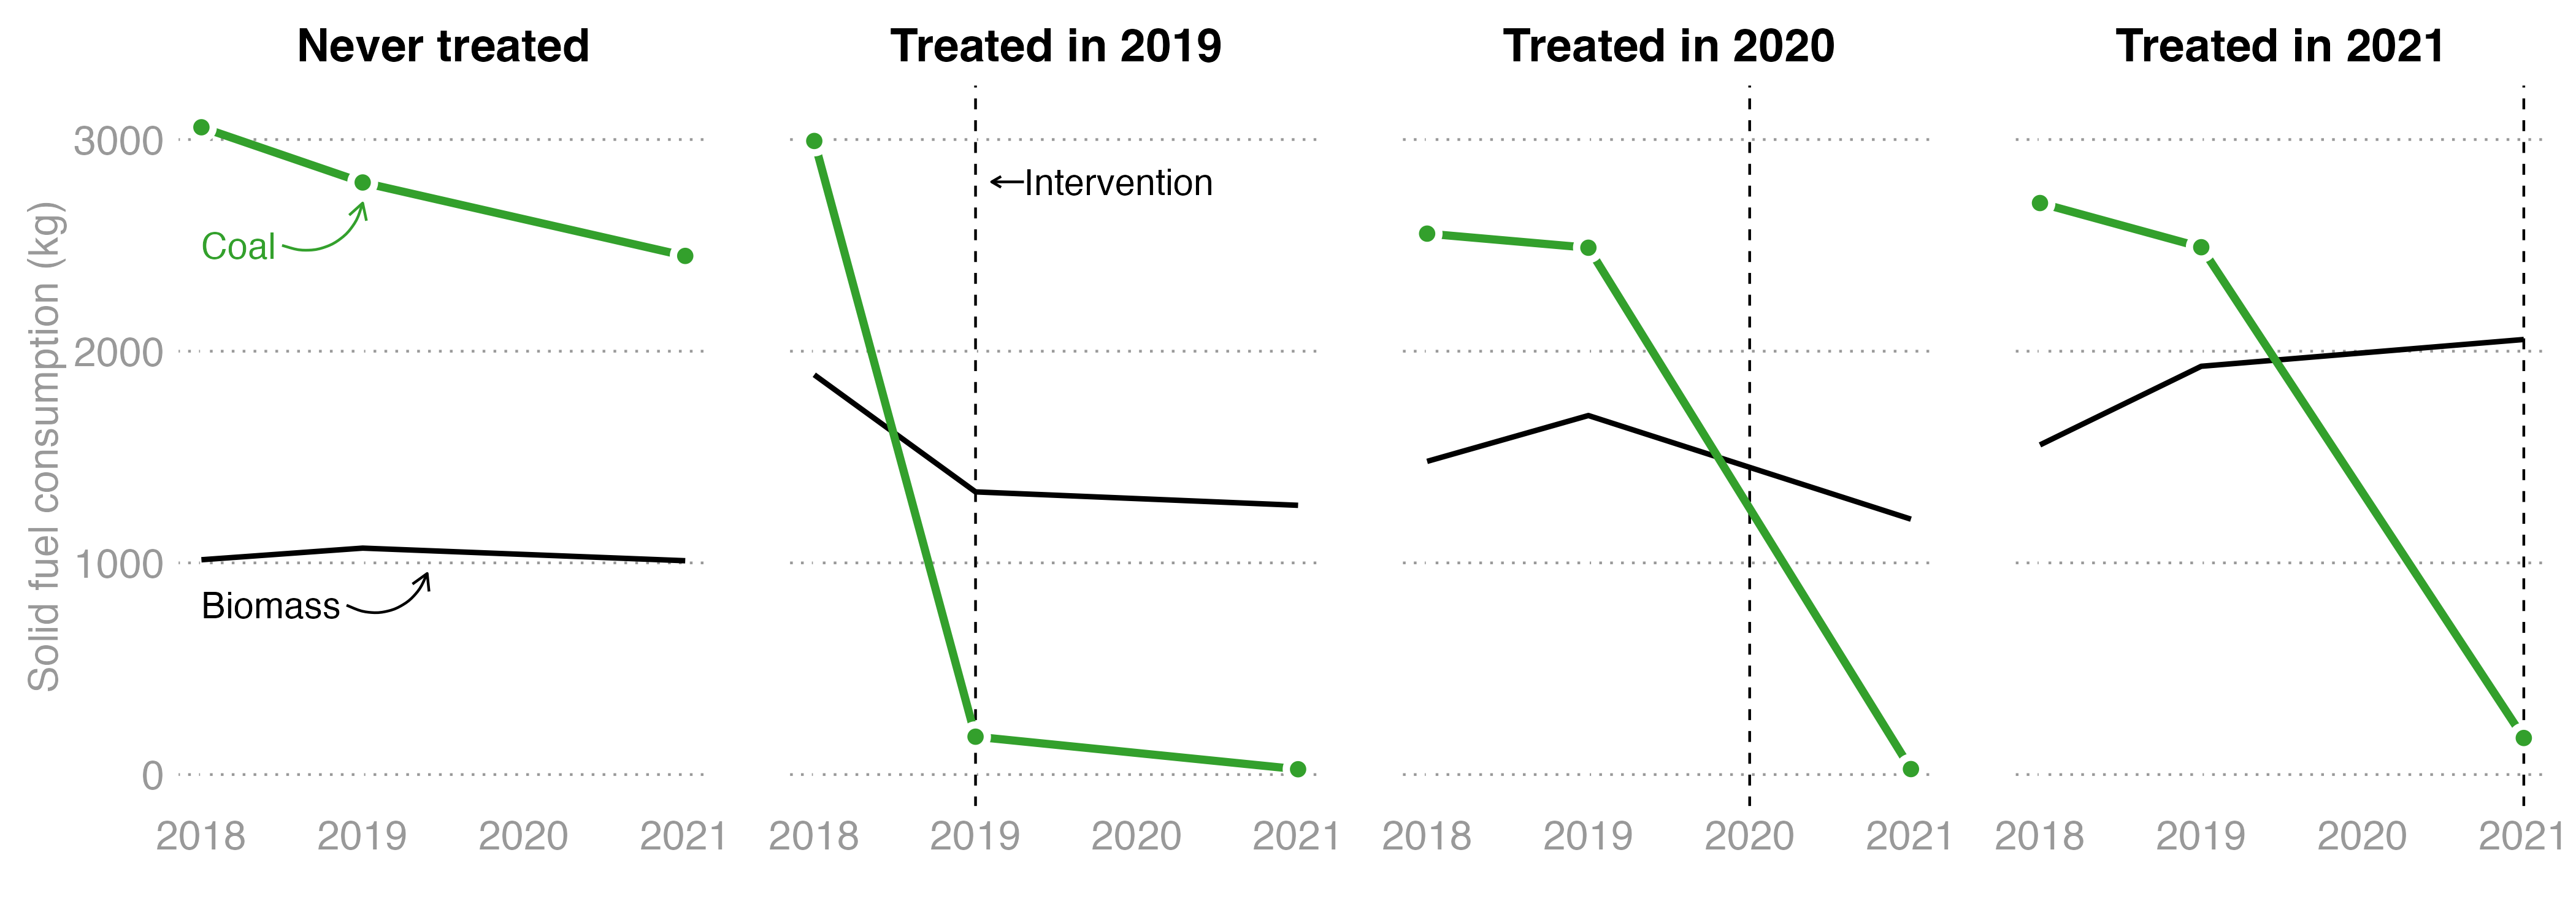
\includegraphics{images/coal-plot.png}

}

}

\end{minipage}%

\end{table}

\textbf{?@tbl-atable1} shows\ldots{}

Compare with Figure \textbackslash ref\{tbl-atable1\}

\hypertarget{about-the-authors}{%
\section*{About the authors}\label{about-the-authors}}
\addcontentsline{toc}{section}{About the authors}

\hypertarget{other-publications}{%
\section*{Other publications}\label{other-publications}}
\addcontentsline{toc}{section}{Other publications}



\end{document}
